\chapter{14/11/17}
LALR(1)
LR(1)

\section{LRm(1)}
\subsection{Esempio}
\begin{tabular}{l}
	$S \rightarrow L=R|R$\\
	$L \rightarrow *R|id$\\
	$R \rightarrow L $\\
\end{tabular}
Lo stato iniziale \'e associato ad una variabile; ottenuto come chiusura (considero gli item LR(1)) 
$S' \rightarrow .S_1\{x_0\}$. \\

\subsubsection{Procedo con la chiusura LR(1)} 
\begin{tabular}{l}
	Equazioni\\
	$x_0 \doteq \{ \$ \}$\\
	$x_1 \doteq \{ x_0 \}$\\
	$x_1 \doteq x_0$\\
	$x_2 \doteq x_0$\\
	$x_3 \doteq x_0$\\
	$x_4 \doteq x_0$\\
	$x_5 \doteq \{ =, x_0 \} \cup \{ x_5 \} \cup \{ x_7 \}$\\
	$x_6 \doteq \{ =, x_0 \} \cup \{ x_5 \} \cup \{ x_7 \}$\\
	$x_7 \doteq \{ x_2 \}$\\
	$x_8 \doteq \{ x_5 \}$\\
	$x_9 \doteq \{ x_5 \} \cup \{ x_7 \}$\\
	$x_10 \doteq \{ x_7 \}$\\
\end{tabular}

\begin{tabular}{l}
	0) Stato 0-esimo
	$S' \rightarrow .S, \{ x_0 \}$\\
	...........................\\
	$S \rightarrow .L=R,\ \{x_0\}$\\
	$S \rightarrow .R,\ \{x_0\}$\\
	$L \rightarrow .*R,\ \{=, x_0\}$\\
	$L \rightarrow .id,\ \{=, x_0\}$\\
	$R \rightarrow .L,\ \{x_0\}$\\
\end{tabular}

\begin{tabular}{l}
	1) Transizione su S ($\rightarrow S$)\\
	$S' \rightarrow S.,\{ x_1 \}$\\
\end{tabular}

\begin{tabular}{l}
	2) Transizione su L\\
	$S \rightarrow L.=R, \{ x_2 \}$\\
	$R \rightarrow L., \{ x_3 \}$\\
\end{tabular}

\begin{tabular}{l}
	3) Transizione su R\\
	$S \rightarrow R., \{ x_4 \}$\\
\end{tabular}

\begin{tabular}{l}
	4) Transizione su *\\
	$L \rightarrow *.R, \{ x_5 \}$\\
	..............................
	$R \rightarrow .L, \{ x_5 \}$\\
	$R \rightarrow .*R, \{ x_5 \}$\\
	$R \rightarrow .id, \{ x_5 \}$\\
\end{tabular}

\begin{tabular}{l}
	5) Transizione su id\\
	$L \rightarrow id., \{ x_6 \}$\\
\end{tabular}

\begin{tabular}{l}
	6) Transizione da 2 su =\\
	$S \rightarrow L=.R, \{ x_7 \}$\\
	...............................\\
	$R \rightarrow .L, \{ x_7 \}$\\
	$L \rightarrow .*R, \{ x_7 \}$\\
	$L \rightarrow .id, \{ x_7 \}$\\
\end{tabular}

\begin{tabular}{l}
	7) Transizione da 4 su R\\
	$L \rightarrow *R., \{ x_8 \}$\\
\end{tabular}

\begin{tabular}{l}
	8) Transizione da 4 su L\\
	$R \rightarrow L., \{ x_9 \}$\\
	Ho un loop sullo stato 4 su * (transizione da 4 in 4)\\
\end{tabular}

\begin{tabular}{l}
	9) Transizione da 6 su R\\
	$S \rightarrow L=R., \{ x_10 \}$\\
	Inserire una L transizione da 6 a 8\\
	Inserire una * transizione da 6 a 4\\
	Inserire una id transizione da 6 a 5\\
\end{tabular}

\begin{tabular}{l}
	Equazioni\\
	$x_0 \doteq \{ \$ \}$\\
	$x_1 \doteq \{ x_0 \}$\\
	$x_1 \doteq x_0$\\
	$x_2 \doteq x_0$\\
	$x_3 \doteq x_0$\\
	$x_4 \doteq x_0$\\
	$x_5 \doteq \{ =, x_0 \} \cup \{ x_5 \} \cup \{ x_7 \}$\\
	$x_6 \doteq \{ =, x_0 \} \cup \{ x_5 \} \cup \{ x_7 \}$\\
	$x_7 \doteq \{ x_2 \}$\\
	$x_8 \doteq \{ x_5 \}$\\
	$x_9 \doteq \{ x_5 \} \cup \{ x_7 \}$\\
	$x_10 \doteq \{ x_7 \}$\\
\end{tabular}

\begin{tcolorbox}\begin{center}
	Controllo le equazioni dalla prima all'ultima e guardo se l'inisieme di destra ho una sola variabile o due di cui una il nodo di destra (self loop).
\end{center}\end{tcolorbox}

	$x_j = \{ x_i \} \cup \{ x_j \} = \{ x_i \}$\\
\begin{tabular}{ll}
	equazione & classe di equivalenza\\
	$x_0 = \{ \$ \}$ & $x_0$\\
	$x_1$ & $x_0$\\
	$x_2$ & $x_0$\\
	$x_3$ & $x_0$\\
	$x_4$ & $x_0$\\

	$x_5 = \{ =, x_0, x_5, x_7 \}$ & $ x_5 $\\
	$x_6 = \{ =, x_0, x_5, x_7 \}$ & $x_0$\\
	$x_7 = \{ \$ \}$ & $ x_6 $\\
	$x_8$ & $x_5$\\
	$x_9$ & $x_0$\\
	$x_10$ & $x_5$\\
\end{tabular}

\begin{tabular}{l}
	$x_0 = \$ $\\
	$x_5 = \{ =, x_0, x_5, x_7 \}$\\
	$x_6 = \{ =, x_0, x_5, x_7 \}$\\
	$x_9 = \{ x_5, x_7 \}$\\
\end{tabular}

\begin{tabular}{l}
	Tolgo i self loop e ridondanze
	$x_0 = \$ $\\
	$x_5 = \{ =, x_0 \}$\\
	$x_6 = \{ =, x_0, x_5 \}$ ($x_7 = x_0$, lo tolgo)\\
	$x_9 = \{ x_5, x_0 \}$\\
\end{tabular}

\begin{center}
	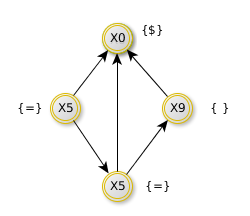
\includegraphics[scale=0.5]{Chapters/Img/l01_01.png}\\
\end{center} 

\begin{tabular}{l}
	$x_0 = \{ \$ \}$\\
	$x_5 = \{ =, \$ \}$\\
	$x_6 = \{ =, \$ \}$\\
	$x_9 = \{ =, \$ \}$\\
\end{tabular}

\section{Algoritmo}
Algoritmo utilizzato da yacc (su dragonbook)
Uso LR0, per ogni item dentro uno stato faccio una chiusura virtuale LR1
Faccio un nuovo grafo e ...

Identifica look ahead generati e propagati, poi fa un grafo e associa ad ogni nodo il look ahead generato

\begin{center}
	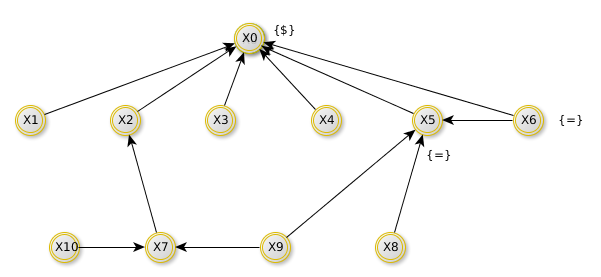
\includegraphics[scale=0.5]{Chapters/Img/l01_02.png}\\
\end{center} 

\begin{tcolorbox}\begin{center}
	Kernel(P) L'insiseme dei kernel item dentro P, proj(P) L'inisieme degli item LR(0) contenuti in P
\end{center}\end{tcolorbox}

\section{Costruzione automa simbolico}
\begin{lstlisting}
	x_0 = new Var()
	vars = {x_0}
	P_0 = closure_1( { [s' -> .s, {x_0} ] } ) //stato iniziale automa
	inizializzare Queue con x_0 = {$}
	States = {P_0}
	porre P_0 come unmarked
	while(c'e' uno stato non marcato P in States){
		marcare P
		foreach(y in V){
			Tmp = emptySet
			foreach([A -> alpha.y beta, delta] <- P){
				aggiungere [A -> alpha.y beta, delta] a Tmp
				if(Tmp != emptySet){
					if( lo stato targhet non e' ancora stato collezionato){
						aggiungere a States una versione simbolica del targhet e aggiungere a Queue una equazione per kernel item in Tmp
					} else {
						raffinare le equazioni delle variabili associate ai kernel item del target
					}
				}
			}
		}
	}
\end{lstlisting}

